%% knit("Foyle_Fisher_t90_modelling.Rnw")

\documentclass[12pt]{article}\usepackage[]{graphicx}\usepackage[]{color}
%% maxwidth is the original width if it is less than linewidth
%% otherwise use linewidth (to make sure the graphics do not exceed the margin)
\makeatletter
\def\maxwidth{ %
  \ifdim\Gin@nat@width>\linewidth
    \linewidth
  \else
    \Gin@nat@width
  \fi
}
\makeatother

\definecolor{fgcolor}{rgb}{0.345, 0.345, 0.345}
\newcommand{\hlnum}[1]{\textcolor[rgb]{0.686,0.059,0.569}{#1}}%
\newcommand{\hlstr}[1]{\textcolor[rgb]{0.192,0.494,0.8}{#1}}%
\newcommand{\hlcom}[1]{\textcolor[rgb]{0.678,0.584,0.686}{\textit{#1}}}%
\newcommand{\hlopt}[1]{\textcolor[rgb]{0,0,0}{#1}}%
\newcommand{\hlstd}[1]{\textcolor[rgb]{0.345,0.345,0.345}{#1}}%
\newcommand{\hlkwa}[1]{\textcolor[rgb]{0.161,0.373,0.58}{\textbf{#1}}}%
\newcommand{\hlkwb}[1]{\textcolor[rgb]{0.69,0.353,0.396}{#1}}%
\newcommand{\hlkwc}[1]{\textcolor[rgb]{0.333,0.667,0.333}{#1}}%
\newcommand{\hlkwd}[1]{\textcolor[rgb]{0.737,0.353,0.396}{\textbf{#1}}}%

\usepackage{framed}
\makeatletter
\newenvironment{kframe}{%
 \def\at@end@of@kframe{}%
 \ifinner\ifhmode%
  \def\at@end@of@kframe{\end{minipage}}%
  \begin{minipage}{\columnwidth}%
 \fi\fi%
 \def\FrameCommand##1{\hskip\@totalleftmargin \hskip-\fboxsep
 \colorbox{shadecolor}{##1}\hskip-\fboxsep
     % There is no \\@totalrightmargin, so:
     \hskip-\linewidth \hskip-\@totalleftmargin \hskip\columnwidth}%
 \MakeFramed {\advance\hsize-\width
   \@totalleftmargin\z@ \linewidth\hsize
   \@setminipage}}%
 {\par\unskip\endMakeFramed%
 \at@end@of@kframe}
\makeatother

\definecolor{shadecolor}{rgb}{.97, .97, .97}
\definecolor{messagecolor}{rgb}{0, 0, 0}
\definecolor{warningcolor}{rgb}{1, 0, 1}
\definecolor{errorcolor}{rgb}{1, 0, 0}
\newenvironment{knitrout}{}{} % an empty environment to be redefined in TeX

\usepackage{alltt}
\usepackage{times}
\usepackage{hyperref}
\usepackage{natbib}
\hypersetup{pdfpagemode=UseNone} % don't show bookmarks on initial view
\hypersetup{colorlinks, urlcolor={blue}}

% revise margins
\setlength{\headheight}{0.0in}
\setlength{\topmargin}{0.0in}
\setlength{\headsep}{0.0in}
\setlength{\textheight}{8.65in}
\setlength{\footskip}{0.35in}
\setlength{\oddsidemargin}{0.0in}
\setlength{\evensidemargin}{0.0in}
\setlength{\textwidth}{6.5in}

\setlength{\parskip}{6pt}
\setlength{\parindent}{0pt}

\title{Preliminary analysis of the \emph{Foyle Fisher} T90 trial data}
\author{For discussion}
\date{}
\IfFileExists{upquote.sty}{\usepackage{upquote}}{}
\begin{document}



\maketitle

\section{Data}

\begin{knitrout}\footnotesize
\definecolor{shadecolor}{rgb}{0.969, 0.969, 0.969}\color{fgcolor}\begin{kframe}
\begin{alltt}
\hlkwd{library}\hlstd{(gdata)} \hlcom{## convert to xlsx}
\hlcom{## read in the Foyle Fisher data}
\hlstd{ff.dat} \hlkwb{<-} \hlkwd{read.xls}\hlstd{(}\hlstr{"../data/Foyle Fisher T90 Trial_edited.xlsx"}\hlstd{,}
                   \hlkwc{sheet} \hlstd{=} \hlstr{"Lengths"}\hlstd{,}
                   \hlkwc{stringsAsFactors} \hlstd{=} \hlnum{FALSE}\hlstd{)}
\hlcom{## Change some names that have spaces}
\hlkwd{names}\hlstd{(ff.dat)[}\hlkwd{names}\hlstd{(ff.dat)} \hlopt{==} \hlstr{"Port...Starboard"}\hlstd{]} \hlkwb{<-} \hlstr{"Port.Starboard"}
\hlkwd{names}\hlstd{(ff.dat)[}\hlkwd{names}\hlstd{(ff.dat)} \hlopt{==} \hlstr{"Control...Experimental"}\hlstd{]} \hlkwb{<-} \hlstr{"Control.Experimental"}
\hlkwd{names}\hlstd{(ff.dat)[}\hlkwd{names}\hlstd{(ff.dat)} \hlopt{==} \hlstr{"Length..cm."}\hlstd{]} \hlkwb{<-} \hlstr{"Length.cm"}
\hlkwd{names}\hlstd{(ff.dat)[}\hlkwd{names}\hlstd{(ff.dat)} \hlopt{==} \hlstr{"Haul.No."}\hlstd{]} \hlkwb{<-} \hlstr{"Haul.No"}

\hlcom{## subset out valid hauls}
\hlstd{ff.dat} \hlkwb{<-} \hlkwd{subset}\hlstd{(ff.dat, Haul.No} \hlopt \hlkwd{c}\hlstd{(}\hlnum{2}\hlstd{,}\hlnum{3}\hlstd{,} \hlnum{6}\hlopt{:}\hlnum{18}\hlstd{))}

\hlcom{## order the data by haul number, species and length class}
\hlstd{ff.dat} \hlkwb{<-} \hlstd{ff.dat[}\hlkwd{with}\hlstd{(ff.dat,} \hlkwd{order}\hlstd{(Haul.No, Species, Length.cm)),]}

\hlcom{## get the subsratio}
\hlstd{ff.dat}\hlopt{$}\hlstd{SUBSRATIO} \hlkwb{<-} \hlkwd{with}\hlstd{(ff.dat, Weight.of.Fish.Measured} \hlopt{/} \hlstd{Total.Weight)}
\hlcom{## not needed generally but it read in ultra small differences}
\hlstd{ff.dat}\hlopt{$}\hlstd{SUBSRATIO} \hlkwb{<-} \hlkwd{round}\hlstd{(ff.dat}\hlopt{$}\hlstd{SUBSRATIO,} \hlnum{10}\hlstd{)}

\hlcom{## Net position}
\hlstd{ff.dat}\hlopt{$}\hlstd{Net.position} \hlkwb{<-} \hlnum{NA}
\hlstd{ff.dat}\hlopt{$}\hlstd{Net.position[ff.dat}\hlopt{$}\hlstd{Control.Experimental} \hlopt{==} \hlstr{"T90 80 mm"} \hlopt{&}
               \hlstd{ff.dat}\hlopt{$}\hlstd{Haul.No} \hlopt \hlkwd{c}\hlstd{(}\hlnum{2}\hlstd{,}\hlnum{3}\hlstd{,}\hlnum{10}\hlopt{:}\hlnum{13}\hlstd{)]} \hlkwb{<-} \hlstr{"Port"}
\hlstd{ff.dat}\hlopt{$}\hlstd{Net.position[ff.dat}\hlopt{$}\hlstd{Control.Experimental} \hlopt{==} \hlstr{"Diamond 80 mm"} \hlopt{&}
               \hlstd{ff.dat}\hlopt{$}\hlstd{Haul.No} \hlopt \hlkwd{c}\hlstd{(}\hlnum{2}\hlstd{,}\hlnum{3}\hlstd{,}\hlnum{10}\hlopt{:}\hlnum{13}\hlstd{)]} \hlkwb{<-} \hlstr{"Starboard"}
\hlstd{ff.dat}\hlopt{$}\hlstd{Net.position[ff.dat}\hlopt{$}\hlstd{Control.Experimental} \hlopt{==} \hlstr{"T90 80 mm"} \hlopt{&}
               \hlstd{ff.dat}\hlopt{$}\hlstd{Haul.No} \hlopt \hlkwd{c}\hlstd{(}\hlnum{6}\hlopt{:}\hlnum{9}\hlstd{,} \hlnum{15}\hlopt{:}\hlnum{18}\hlstd{)]} \hlkwb{<-} \hlstr{"Starboard"}
\hlstd{ff.dat}\hlopt{$}\hlstd{Net.position[ff.dat}\hlopt{$}\hlstd{Control.Experimental} \hlopt{==} \hlstr{"Diamond 80 mm"} \hlopt{&}
               \hlstd{ff.dat}\hlopt{$}\hlstd{Haul.No} \hlopt \hlkwd{c}\hlstd{(}\hlnum{6}\hlopt{:}\hlnum{9}\hlstd{,} \hlnum{15}\hlopt{:}\hlnum{18}\hlstd{)]} \hlkwb{<-} \hlstr{"Port"}

\hlcom{## subset by species}
\hlstd{plaice.dat} \hlkwb{<-} \hlkwd{subset}\hlstd{(ff.dat, Species} \hlopt{==} \hlstr{"Plaice"}\hlstd{)}
\hlstd{whit.dat} \hlkwb{<-} \hlkwd{subset}\hlstd{(ff.dat, Species} \hlopt{==} \hlstr{"Whiting"}\hlstd{)}
\hlstd{had.dat} \hlkwb{<-} \hlkwd{subset}\hlstd{(ff.dat, Species} \hlopt{==} \hlstr{"Haddock"}\hlstd{)}
\end{alltt}
\end{kframe}
\end{knitrout}

\begin{knitrout}\footnotesize
\definecolor{shadecolor}{rgb}{0.969, 0.969, 0.969}\color{fgcolor}\begin{kframe}
\begin{alltt}
\hlcom{## get count per length bin per haul by experimental gear}
\hlkwd{library}\hlstd{(reshape)}

\hlcom{## variables to keep }
\hlstd{vars2keep} \hlkwb{<-} \hlkwd{c}\hlstd{(}\hlstr{"Control.Experimental"}\hlstd{,} \hlstr{"Length.cm"}\hlstd{,} \hlstr{"Haul.No"}\hlstd{,} \hlstr{"Count"}\hlstd{)}

\hlcom{## melt the data frame}
\hlstd{plaice.dat.melt} \hlkwb{<-} \hlkwd{melt}\hlstd{(plaice.dat[, vars2keep],}
                    \hlkwc{id} \hlstd{=} \hlkwd{c}\hlstd{(}\hlstr{"Control.Experimental"}\hlstd{,} \hlstr{"Length.cm"}\hlstd{,} \hlstr{"Haul.No"}\hlstd{))}

\hlcom{## re-form the dataframe in required format }
\hlstd{plaice.dat.cast} \hlkwb{<-} \hlkwd{cast}\hlstd{(plaice.dat.melt, Length.cm} \hlopt{+} \hlstd{Haul.No} \hlopt{~} \hlstd{Control.Experimental}  \hlopt{+} \hlstd{variable)}
\hlstd{plaice.dat.cast} \hlkwb{<-} \hlstd{plaice.dat.cast[}\hlkwd{order}\hlstd{(plaice.dat.cast}\hlopt{$}\hlstd{Haul.No, plaice.dat.cast}\hlopt{$}\hlstd{Length.cm), ]}
\hlstd{plaice.dat.cast[}\hlkwd{is.na}\hlstd{(plaice.dat.cast)]} \hlkwb{<-} \hlnum{0}

\hlcom{## show the first few rows}
\hlkwd{head}\hlstd{(plaice.dat.cast,} \hlnum{2}\hlstd{)}
\end{alltt}
\begin{verbatim}
##   Length.cm Haul.No Diamond 80 mm_Count T90 80 mm_Count
## 1        17       2                   1               0
## 2        18       2                   1               2
\end{verbatim}
\begin{alltt}
\hlcom{## format the subsampling ratio similarly}
\hlstd{vars2keep} \hlkwb{<-} \hlkwd{c}\hlstd{(}\hlstr{"Control.Experimental"}\hlstd{,} \hlstr{"Haul.No"}\hlstd{,} \hlstr{"SUBSRATIO"}\hlstd{)}
\hlstd{subs.melt} \hlkwb{<-} \hlkwd{melt}\hlstd{(}\hlkwd{unique}\hlstd{(plaice.dat[, vars2keep]),} \hlkwc{id} \hlstd{=} \hlkwd{c}\hlstd{(}\hlstr{"Control.Experimental"}\hlstd{,} \hlstr{"Haul.No"}\hlstd{))}
\hlstd{subs.cast} \hlkwb{<-} \hlkwd{cast}\hlstd{(subs.melt, Haul.No}  \hlopt{~} \hlstd{Control.Experimental} \hlopt{+} \hlstd{variable)}

\hlcom{## get net position of each}
\hlstd{vars2keep} \hlkwb{<-} \hlkwd{c}\hlstd{(}\hlstr{"Control.Experimental"}\hlstd{,} \hlstr{"Haul.No"}\hlstd{,} \hlstr{"Net.position"}\hlstd{)}
\hlstd{netpos.melt} \hlkwb{<-} \hlkwd{melt}\hlstd{(}\hlkwd{unique}\hlstd{(plaice.dat[, vars2keep]),} \hlkwc{id} \hlstd{=} \hlkwd{c}\hlstd{(}\hlstr{"Control.Experimental"}\hlstd{,} \hlstr{"Haul.No"}\hlstd{))}
\hlstd{netpos.cast} \hlkwb{<-} \hlkwd{cast}\hlstd{(netpos.melt, Haul.No}  \hlopt{~} \hlstd{Control.Experimental} \hlopt{+} \hlstd{variable)}

\hlcom{## merge counts and subsampling ratio back together }
\hlstd{plaice.dat.cast0} \hlkwb{<-} \hlkwd{merge}\hlstd{(plaice.dat.cast, subs.cast,} \hlkwc{by} \hlstd{=} \hlstr{"Haul.No"}\hlstd{,} \hlkwc{all.x} \hlstd{=} \hlnum{TRUE}\hlstd{)}

\hlstd{plaice.dat.cast} \hlkwb{<-} \hlkwd{merge}\hlstd{(plaice.dat.cast0, netpos.cast,} \hlkwc{by} \hlstd{=} \hlstr{"Haul.No"}\hlstd{,} \hlkwc{all.x} \hlstd{=} \hlnum{TRUE}\hlstd{)}

\hlcom{## show first few lines}
\hlkwd{head}\hlstd{(plaice.dat.cast,} \hlnum{2}\hlstd{)}
\end{alltt}
\begin{verbatim}
##   Haul.No Length.cm Diamond 80 mm_Count T90 80 mm_Count
## 1       2        17                   1               0
## 2       2        18                   1               2
##   Diamond 80 mm_SUBSRATIO T90 80 mm_SUBSRATIO Diamond 80 mm_Net.position
## 1               0.7515528           0.5742188                  Starboard
## 2               0.7515528           0.5742188                  Starboard
##   T90 80 mm_Net.position
## 1                   Port
## 2                   Port
\end{verbatim}
\begin{alltt}
\hlcom{## Extract the matrix of counts}
\hlstd{count.vars} \hlkwb{<-} \hlkwd{c}\hlstd{(}\hlstr{"T90 80 mm_Count"}\hlstd{,} \hlstr{"Diamond 80 mm_Count"}\hlstd{)}
\hlstd{plaice.count.mat} \hlkwb{<-} \hlkwd{as.matrix}\hlstd{(plaice.dat.cast[, count.vars])}

\hlcom{## Extract the matrix of subsampling ratios}
\hlstd{subsratio.vars} \hlkwb{<-} \hlkwd{c}\hlstd{(}\hlstr{"T90 80 mm_SUBSRATIO"}\hlstd{,} \hlstr{"Diamond 80 mm_SUBSRATIO"}\hlstd{)}
\hlstd{subsratio.mat} \hlkwb{<-} \hlkwd{as.matrix}\hlstd{(plaice.dat.cast[, subsratio.vars])}

\hlcom{## Create the offset}
\hlstd{offset.mat} \hlkwb{<-} \hlkwd{log}\hlstd{(}\hlkwd{apply}\hlstd{(subsratio.mat,} \hlnum{2}\hlstd{,} \hlkwc{FUN} \hlstd{=}
                        \hlkwa{function}\hlstd{(}\hlkwc{zz}\hlstd{)\{zz}\hlopt{/}\hlstd{subsratio.mat[,}\hlnum{1}\hlstd{]\}))}
\end{alltt}
\end{kframe}
\end{knitrout}

\section{Plots}


Plot the data 
\begin{knitrout}\footnotesize
\definecolor{shadecolor}{rgb}{0.969, 0.969, 0.969}\color{fgcolor}\begin{kframe}
\begin{alltt}
\hlkwd{library}\hlstd{(ggplot2)}

\hlcom{## Get the proportions}
\hlstd{raised.count.mesh} \hlkwb{<-} \hlkwd{as.matrix}\hlstd{(plaice.dat.cast[, count.vars])} \hlopt{/} \hlstd{subsratio.mat}

\hlstd{prop.mesh} \hlkwb{<-} \hlkwd{prop.table}\hlstd{(raised.count.mesh,} \hlkwc{margin} \hlstd{=} \hlnum{1}\hlstd{)}
\hlstd{m} \hlkwb{<-} \hlkwd{dim}\hlstd{(prop.mesh)[}\hlnum{1}\hlstd{]}

\hlstd{prop.mesh.df} \hlkwb{<-} \hlkwd{data.frame}\hlstd{(}
                  \hlkwc{Length.cm} \hlstd{= plaice.dat.cast}\hlopt{$}\hlstd{Length.cm,}
                  \hlkwc{Haul.No} \hlstd{= plaice.dat.cast}\hlopt{$}\hlstd{Haul.No,}
                  \hlkwc{proportion} \hlstd{=} \hlkwd{c}\hlstd{(prop.mesh[,}\hlnum{1}\hlstd{]),}
                  \hlkwc{total.count} \hlstd{=} \hlkwd{rowSums}\hlstd{(raised.count.mesh))}

\hlstd{plaice.agg.count} \hlkwb{<-} \hlkwd{aggregate}\hlstd{(plaice.dat.cast[,} \hlkwd{c}\hlstd{(}\hlstr{"T90 80 mm_Count"}\hlstd{,} \hlstr{"Diamond 80 mm_Count"}\hlstd{)],} \hlkwd{list}\hlstd{(}\hlkwc{Length.cm} \hlstd{= plaice.dat.cast}\hlopt{$}\hlstd{Length.cm), sum)}
\hlstd{plaice.agg.count}\hlopt{$}\hlstd{proportion} \hlkwb{<-} \hlkwd{prop.table}\hlstd{(}\hlkwd{as.matrix}\hlstd{(plaice.agg.count[,}\hlnum{2}\hlopt{:}\hlnum{3}\hlstd{]),} \hlkwc{margin} \hlstd{=} \hlnum{1}\hlstd{)[,}\hlnum{1}\hlstd{]}

\hlstd{plaice.plot} \hlkwb{<-} \hlkwd{ggplot}\hlstd{(prop.mesh.df,} \hlkwd{aes}\hlstd{(}\hlkwc{x} \hlstd{= Length.cm,} \hlkwc{y} \hlstd{= proportion))} \hlopt{+}
  \hlkwd{geom_point}\hlstd{(}\hlkwc{colour} \hlstd{=} \hlstr{"#FF9900"}\hlstd{,} \hlkwc{alpha} \hlstd{=} \hlnum{0.5}\hlstd{,} \hlkwd{aes}\hlstd{(}\hlkwc{size} \hlstd{=} \hlkwd{log}\hlstd{(total.count)))} \hlopt{+}
  \hlkwd{ylab}\hlstd{(}\hlstr{"Proportion of Plaice in T90"}\hlstd{)} \hlopt{+} \hlkwd{theme}\hlstd{(}\hlkwc{legend.position} \hlstd{=} \hlstr{"none"}\hlstd{)} \hlopt{+}
  \hlkwd{geom_line}\hlstd{(}\hlkwc{data} \hlstd{= plaice.agg.count,} \hlkwc{colour} \hlstd{=} \hlstr{"grey"}\hlstd{)}

\hlstd{plaice.plot}
\end{alltt}
\end{kframe}\begin{figure}
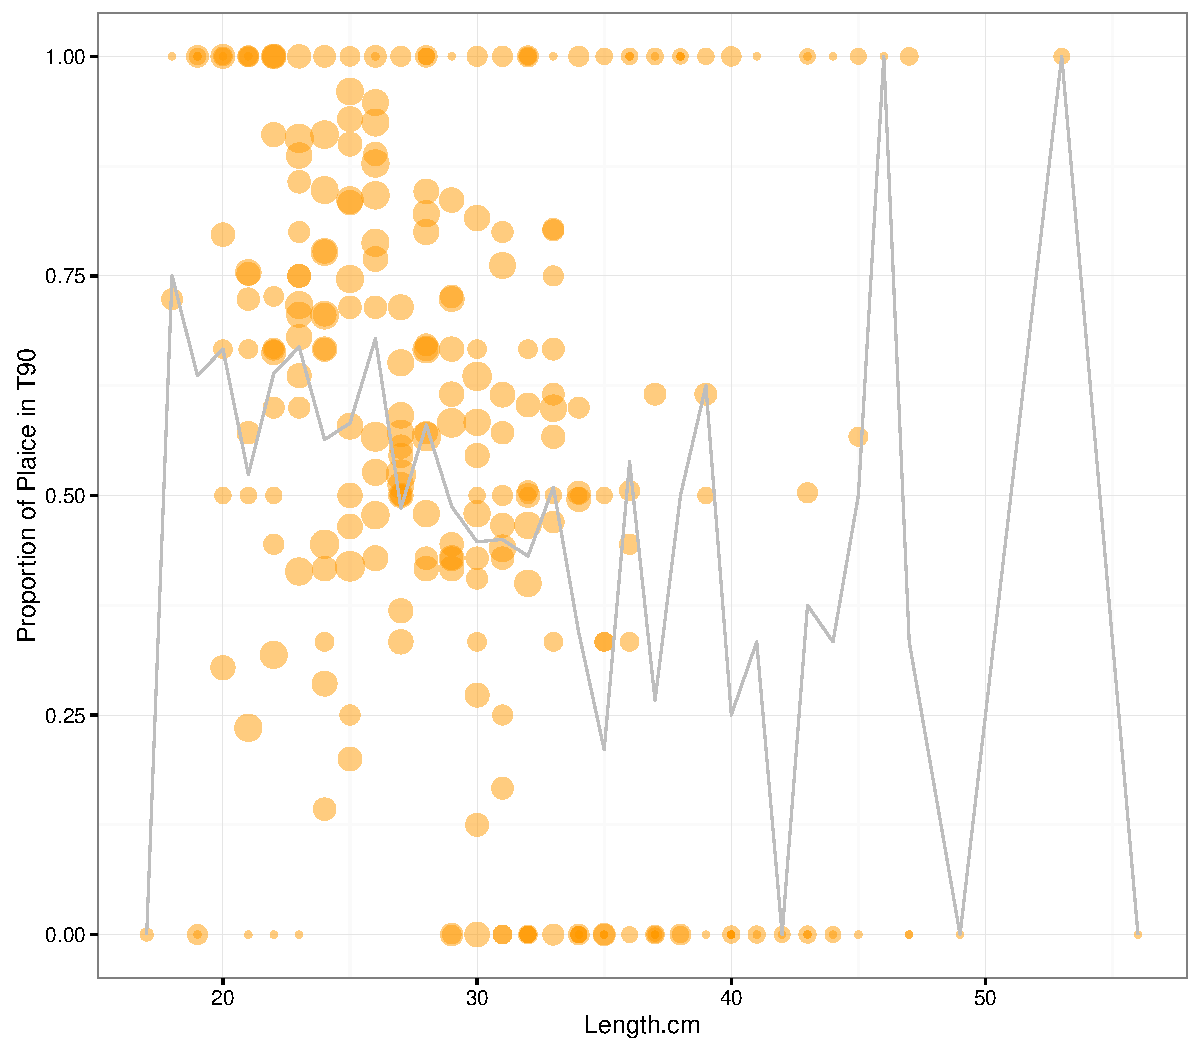
\includegraphics[width=\maxwidth]{figure/unnamed-chunk-4-1} \caption[Proportion of plaice catch retained per haul]{Proportion of plaice catch retained per haul. Each point represents the proportion of the plaice catch (in number) per haul and length class retained in the T90 experimental gear. The size of the point is proportional to the log of the count.}\label{fig:unnamed-chunk-4}
\end{figure}


\end{knitrout}



\end{document}
